%%%%%%%%%%%%%%%%%%%%%%%%%%%%%%%%%%%%%%%%%
% Short Sectioned Assignment
% LaTeX Template
% Version 1.0 (5/5/12)
%
% This template has been downloaded from:
% http://www.LaTeXTemplates.com
%
% Original author:
% Frits Wenneker (http://www.howtotex.com)
%
% License:
% CC BY-NC-SA 3.0 (http://creativecommons.org/licenses/by-nc-sa/3.0/)
%
%%%%%%%%%%%%%%%%%%%%%%%%%%%%%%%%%%%%%%%%%

%----------------------------------------------------------------------------------------
%	PACKAGES AND OTHER DOCUMENT CONFIGURATIONS
%----------------------------------------------------------------------------------------

\documentclass[letterpaper, fontsize=11pt]{scrartcl} 

\usepackage[T1]{fontenc} % Use 8-bit encoding that has 256 glyphs
\usepackage{fourier} % Use the Adobe Utopia font for the document - comment this line to return to the LaTeX default
\usepackage[english]{babel} % English language/hyphenation
\usepackage{amsmath,amsfonts,amsthm} % Math packages

\usepackage{lipsum} % Used for inserting dummy 'Lorem ipsum' text into the template

\usepackage{sectsty} % Allows customizing section commands
\allsectionsfont{\centering \normalfont\scshape} % Make all sections centered, the default font and small caps

\usepackage{fancyhdr} % Custom headers and footers
\usepackage{graphicx}
\usepackage{mcode}

\pagestyle{fancyplain} % Makes all pages in the document conform to the custom headers and footers
\fancyhead{} % No page header - if you want one, create it in the same way as the footers below
\fancyfoot[L]{\textit{CME 102 Winter '17-'18}} % Empty left footer
\fancyfoot[C]{\thepage} % Empty center footer
\fancyfoot[R]{Tim Anderson} % Page numbering for right footer
\renewcommand{\headrulewidth}{0pt} % Remove header underlines
\renewcommand{\footrulewidth}{0pt} % Remove footer underlines
\setlength{\headheight}{13.6pt} % Customize the height of the header

\numberwithin{equation}{section} % Number equations within sections (i.e. 1.1, 1.2, 2.1, 2.2 instead of 1, 2, 3, 4)
\numberwithin{figure}{section} % Number figures within sections (i.e. 1.1, 1.2, 2.1, 2.2 instead of 1, 2, 3, 4)
\numberwithin{table}{section} % Number tables within sections (i.e. 1.1, 1.2, 2.1, 2.2 instead of 1, 2, 3, 4)

\setlength\parindent{0pt} % Removes all indentation from paragraphs - comment this line for an assignment with lots of text
\begin{document}

%----------------------------------------------------------------------------------------
%	TITLE SECTION
%----------------------------------------------------------------------------------------

\newcommand{\horrule}[1]{\rule{\linewidth}{#1}} % Create horizontal rule command with 1 argument of height

%----------------------------------------------------------------------------------------
%	PROBLEM 1
%----------------------------------------------------------------------------------------

\section*{Week 5 Section Problems}
\par Solve the following problems. If initial conditions are given, solve for all constants of integration. It is okay to leave answers in implicit form or with unsolved integrals. 

\begin{enumerate}
\item $x y''  + 2y' + x  = 1$, $y(1) = 2$, $y'(1) = 1$ \par
\textbf{Solution} \newline
Substitute $z = y'$:
$$ xz' + 2z + x = 1$$
$$ z = \frac{C}{x^2} - \frac{x}{3} + \frac{1}{2}$$
$$ y' = \frac{C}{x^2} - \frac{x}{3} + \frac{1}{2}$$
$$ y = \frac{c_1}{x} + c_2 - \frac{x^2}{6} + \frac{x}{2}$$
\begin{center} $ y(1) = 2 = c_1 + c_2 - \frac{1}{3}$, $\frac{7}{3} = c_1 + c_2$ \end{center}
$$y' = \frac{c_1}{x^2} - \frac{x}{3} + \frac{1}{2}$$
$$y'(1) = 1 = -c_1 - \frac{1}{3} + \frac{1}{2}$$
\begin{center} $c_1 = -\frac{5}{6}$, $c_2 = \frac{3}{2}$\end{center}
$$y(x) = -\frac{5}{6x} + \frac{3}{2} - \frac{x^2}{6} + \frac{x}{2}$$

\item $y'' - y'y = 0$\par
\textbf{Solution} \newline
This is a "missing x" nonlinear ODE. Subsitute $v = y'$ and solve:
$$y'' = v\frac{dv}{dy}$$
$$v\frac{dv}{dy} + vy = 0$$
$$dv = -y dy$$
$$v = \frac{-y^2}{2} + c_1$$
$$\frac{dy}{dx} = \frac{y^2}{2}+c_1$$
$$\frac{dy}{dx} = \frac{y^2}{2}+c_1$$
$$\frac{dy}{y^2/2 + c_1} = dx$$
$$\frac{\sqrt{2}}{\sqrt{c_1}}tan^{-1}(y/\sqrt{c_1}) = x + c_2$$
$$y = \sqrt{c_1} tan(\sqrt{c_1}x + c_2)$$

%\item $2x^2y'' + xy' + y = 0$ \par
%\textbf{Solution} \newline
%This is a Cauchy-Euler equation. We use a trial solution $y = x^m$:
%$$2x^2(m)(m-1)(x^{m-2}) + x(m)(x^{m-1}) + x^m = 0$$
%$$2m(m-1) + m + 1 = 0$$
%$$m = \frac{1}{4} \pm \frac{\imath\sqrt{7}}{4}$$
%Which from the form of the solution for a Cauchy-Euler equation, we have:
%$$y(x) = c_1 x^{1/4} cos\bigg(\frac{\sqrt{7}}{4} ln(x)\bigg) + c_2 x^{1/4} sin\bigg(\frac{\sqrt{7}}{4} ln(x)\bigg)$$


\item $\frac{1}{3}x^2y'' + xy' + \frac{1}{3}y = 0 $, $y(1) = 1$, $y'(1) = 1$ \par
\textbf{Solution} \newline
This is also a Cauchy-Euler equation. We thus use a trial solution $y = x^m$:
$$x^2y'' + 3xy' + y = 0 $$
$$m(m-1) + 3m + 1 = 0 $$
$$ m = -1$$
$$y(x) = x^{-1}(c_1 ln(x) + c_2)$$
Applying initial conditions:
$$y(1) = 1 = c_2$$
$$y'= \frac{d}{dx}\Big(\frac{c_1 ln(x)}{x} + \frac{1}{x}\Big) = \frac{c_1 - 1}{x^2} - \frac{c_1 ln(x)}{x^2}$$
$y'(1) = 1 = c_1 - 1$, $c_1 = 2$
$$y(x) = x^{-1}(2 ln(x) + 1)$$
\item \textbf{ode45:} For the following system, write a function to evaluate the derivatives, and then write the function call to ode45 to store the numerical solution over the range $0\leq t \leq 10$. Be sure to pass $\alpha$ as a parameter into the derivative function.
$$ \dot{x}  =  2x + 3y$$
$$\dot{y} = x - \alpha y$$
$$ x(0) = y(0) = 1$$
\textbf{Solution} \newline
The derivative function would be:
\begin{lstlisting} 
function yp = f(t,y,a)
	yp = zeros(2,1);
	yp(1) = 2*y(1) + 3*y(2);
	yp(2) = y(1) - a*y(2);
end
\end{lstlisting}

and the function call is:
\begin{lstlisting}
[T Y] = ode45(@(t,y) yp(t,y,a), [0 10], [1 1]);
\end{lstlisting}
\item The red and green lines in the plot below are the numerical solution to a coupled system of ODEs, and the blue line is a plot of step size taken by ode45 over the domain. What is the relationship between the step size and numerical solution? \textit{Hint:} Think about the derivative of the functions. \newline
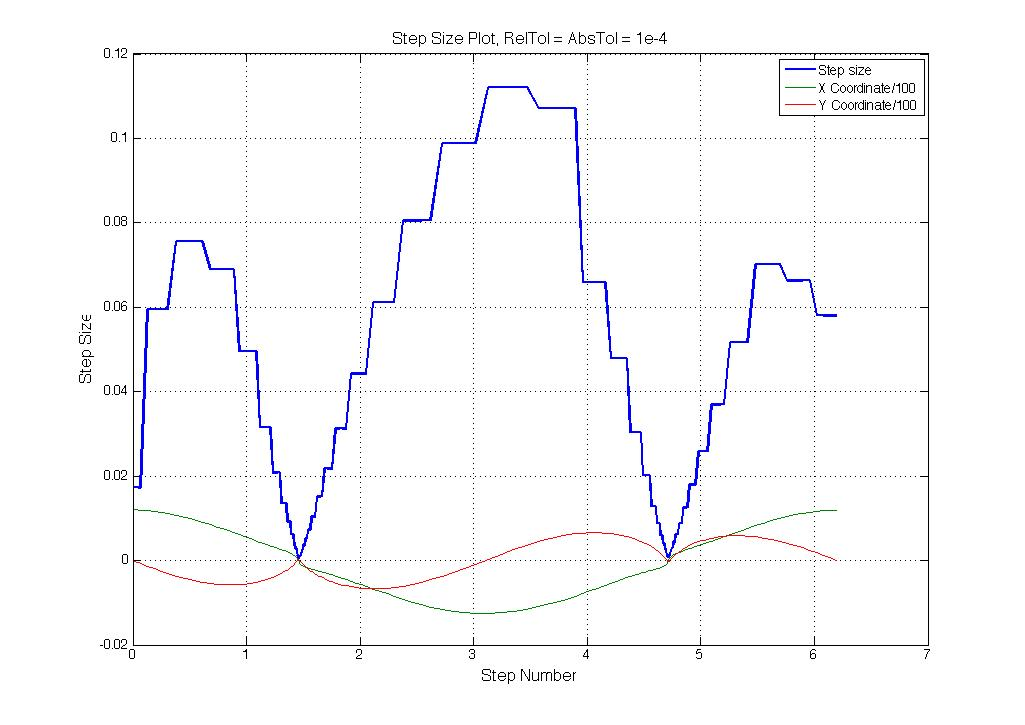
\includegraphics[width=\textwidth]{section5_1.jpg}
\textbf{Solution:} The step size is inversely proportional to the absolute value of the derivative of the fastest-changing function. In this case, the red line is the faster changing function, so the step size is very small when the red line changes quickly (particularly at the non-differentiable points) and larger when the red line is not changing as quickly. The green line is smooth and has small first derivative, so although the step size is determined by the rate of change in the system as a whole, the green line does not dominate the red line. \par
\textbf{Remark:} remember that ode45 is an adaptive step size solver, so it changes the step size based on the rate of change and smoothness of the function. This is different from the RK4 function you write for the homework in this class. RK4 is a discritization scheme, whereas ode45 is a function with built-in algorithms to determine the step size. In fact, RK4 is the numerical scheme underlying ode45, but ode45 uses a 5th-order discritization scheme to check if the step size being used with the 4th order RK4 scheme is accurate enough. (4 and 5 order schemes, hence "ode45".)

\end{enumerate}

%----------------------------------------------------------------------------------------

\end{document}